\chapter{Apéndice}

En esta sección, se pueden encontrar diversos tipos de contenido, tales como datos brutos, códigos fuente, resultados detallados, diagramas extensivos, y cualquier otra documentación que, aunque esencial, podría interrumpir el flujo de lectura si se incluyera en el cuerpo principal del texto. El objetivo del apéndice es facilitar al lector interesado un acceso directo a estos materiales, permitiéndole profundizar en los aspectos técnicos o metodológicos del proyecto sin sobrecargar el texto principal.

\section{Circuitos}\label{ApendiceDiseñoEsquematico}

Los circuitos son una parte fundamental de cualquier proyecto de electrónica, y su correcto diseño y funcionamiento son esenciales para el éxito de la implementación. En esta sección, se incluyen los esquemáticos de los circuitos utilizados en el proyecto, así como cualquier información adicional relevante para su comprensión y reproducción.

Todos los circuitos que componen el proyecto se han originado de versiones anteriores de los mismos, y han sido adaptados y mejorados para cumplir con los requisitos específicos de la presente implementación.

\subsection{Esp32S3 con Agujero}\label{ApendiceEsp32Hole}
Dado que el componente ESP32S3 es un componente de montaje superficial y este posee una parte inferior con los \glsnocase{Pads} de soldadura a tierra totalmente debajo del componente, se ha decidido modificar el componente (Parte de Eagle) para que sea más sencillo de soldar. Para ello, se ha añadido un agujero en la parte inferior del componente para que los \glsnocase{Pads} de soldadura sean visibles desde el otro lado de la placa.

Para ello vamos a ir a Eagle e importaremos la librería de ESP32S3. Iremos a editar el \glsnocase{Footprint} y donde están los terminales inferiores en mitad del dispositivo vamos a sustituirlos por un agujero de soldadura de las mismas dimensiones. 

Todos los pasos han sido realizados siguiendo el tutorial descrito en la asignatura de Circuitos Impresos. Una descripción breve de los pasos a seguir es la siguiente.

\begin{enumerate}
    \item Abrir o Crear una Librería
    Abra EAGLE y cree una nueva librería con el nombre deseado (en nuestro caso, ``ESP32S3HOLE'').
    \item Seleccionar y Nombrar el Device
    Seleccione ``Device'' y asígnele un nombre (por ejemplo, ``ESP32S3HOLE'').
    \item Crear el Símbolo del Componente
    Dibuje el símbolo del componente y añada los pines necesarios, asignando nombres a cada pin según corresponda. Trace el diseño del símbolo de acuerdo con sus especificaciones. En nuestro caso podremos encontrar las dimensiones, pines y demás en la hoja de datos del componente ESP32S3 \cite{ESP32S3Datasheet}.
    \item Usar un Package Existente
    Para ello, abra la librería en edición, vaya a la librería en el menú principal, elija el componente, haga clic con el botón derecho y seleccione la opción ``Copiar a Librería''.
    \item Editar el \glsnocase{Footprint}
    Abra la librería en edición, seleccione el componente, haga clic con el botón derecho y seleccione la opción ``Edit Package''. A continuación, edite el \glsnocase{Footprint} según sus especificaciones.
    Este paso es el más importante, ya que aquí es donde se añadirá el agujero de soldadura. Para ello, seleccione los pines inferiores del componente y sustitúyalos por un agujero de soldadura de las mismas dimensiones. Asegúrese de que el agujero de soldadura esté correctamente alineado con los pines del componente.
    Ahora que el \glsnocase{Footprint} ha sido modificado, guarde los cambios y cierre la ventana de edición.
    \item Unir Pines
    Para unir los pines del símbolo del componente con los pines del \glsnocase{Footprint}, seleccione el componente en la librería en edición, haga clic con el botón derecho y seleccione la opción ``Connect Package''.
    \item Añadir Atributos
    Añada los atributos necesarios al componente, como el valor, la descripción, etc.
\end{enumerate}

De forma que quedara como podemos ver en la figura \ref{fig:ESP32S3HOLE}.

\begin{figure}[H]
    \centering
    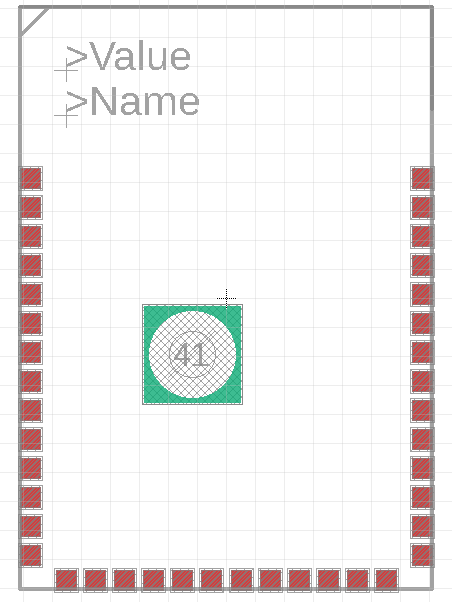
\includegraphics[width=0.7\textwidth]{imagenes/Capitulos/Cap13/ESP32S3HOLE.png}
    \caption{Imagen de la ESP32S3 modificada}
\end{figure}\label{fig:ESP32S3HOLE}

\section{PCB}\label{ApendicePCB}

\subsection{Dimensiones físicas}
Dado que el proyecto se va a realizar en una placa de madera, y esta contenga todos los elementos, y que la placa de madera va a ser fresada con una fresadora CNC, se ha decidido dejar márgenes de 1 mm en cada lado de la placa. Además de añadir un margen extra a la \gls{PCB} para que pueda ser atornillada más fácilmente.

En la figura \ref{fig:PlanoSeparacionMadera} podemos ver en rojo el borde de la \gls{PCB} y la línea más próxima, en negro, la madera. Se ha dejado medio milímetro de margen para las máquinas \gls{CNC} y de fabricación de \gls{PCB}. Los marcadores de los interruptores generados por el software de la sección \ref{CreacionPlanoDistribucion} se ha dejado en verde.

\begin{figure}[H]
    \centering
    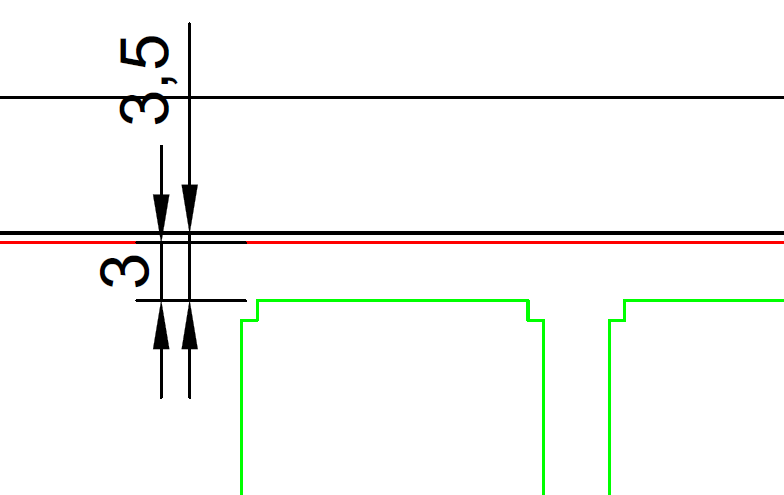
\includegraphics[width=0.8\textwidth]{imagenes/Capitulos/Cap05/AcotadoPCBMadera.png}
    \caption{Imagen del plano acotado del espacio entre las \glsnocase{Keycaps} y la madera.}
    \label{fig:PlanoSeparacionMadera}
\end{figure}

También la idea siempre ha sido ajustar las dimensiones de la carcasa y \gls{PCB} para que no se viera la \gls{PCB} una vez que el teclado tuviese las \glsnocase{Keycaps} puestas, esto ya que al no haber \glsnocase{Plate} si dejáramos mucho hueco, esta parte se vería peor estéticamente. Por eso, uno de los objetivos es intentar que la carcasa esté lo más cerca de las \glsnocase{Keycaps}.
\newpage

\section{Programación}
\subsection{Código fuente}\label{ApendiceCodigoFuente}

Todo el código fuente del proyecto se encuentra disponible en el repositorio de GitHub del proyecto \cite{ModernWoodGitHub}. En este repositorio, se pueden encontrar todos los archivos necesarios para la implementación del proyecto, incluyendo el código fuente, los esquemáticos, las librerías, y cualquier otra documentación relevante. Este GitHub tiene todo el contenido que se ha necesitado para la realización del proyecto. Cualquier persona que quiera realizar el proyecto puede descargarse el código y los esquemáticos y realizarlo sin problemas. Además de servirse de la documentación que se ha ido generando a lo largo del proyecto para su montaje y fabricación.

\subsection{Estructuras}

En esta sección se describen las estructuras de datos y funciones más relevantes utilizadas en el proyecto. Estas van desde la configuración de la \gls{EEPROM}, hasta la configuración de los distintos modos de funcionamiento del teclado. Las variables de estado o las clases principales que se han utilizado en el proyecto. Así como donde poder encontrar estas estructuras en el código fuente.
\subsubsection{Variables de estado}

Estas variables son las que se han utilizado para saber el estado del teclado. Estas variables se han ido creando a lo largo del proyecto y se han ido añadiendo a medida que se iban necesitando. Estas variables se encuentran en el archivo de ModernWood/ModernWood/include/ModernWood.h. Un ejemplo de estas variables se puede ver en el código \ref{code:VariablesEstado}.

\begin{lstlisting}[style=console, language=bash, caption={Variables de estado del teclado}, label={code:VariablesEstado}]
    // Variable to switch between keyboard and display mode
    extern bool volatile WorkingAsKeyboard;
    extern bool volatile interrupted_FN;

    // Variables to know the state of the keyboard
    extern bool displayChanged; //Main display changed (to update the display in the main loop)
    extern bool volatile isUSBConnected;
    extern bool volatile isBLEConnected;
    extern bool isBluetoothOn;
    extern bool connectionChanged;
    
    // Battery energy save mode variables
    extern bool goingToSleep;
    extern bool Sleeping;
    extern bool timerSetupDone;

    //Battery level (need to update the display when it changes)
    extern bool batteryLevelChanged;
    
    extern bool inExternalFunctionMode; //To know if we are in the external function mode
    extern bool executingCustomFunction; //To know if we are executing a custom function
    //If there is a actual function begin exectued, which is the row and col of the key
    extern int actualFunctionRow; 
    extern int actualFunctionCol;

    //To know if we are in the menu and which option is selected
    extern int option_selected;
    extern int option_selected_submenu;

\end{lstlisting}

\subsubsection{Configuración EEPROM} \label{ApendiceConfigEEPROM}
Una de las estructuras más importantes que se han utilizado en el proyecto es la estructura de la configuración a guardar en la memoria \gls{EEPROM}. Esta se compone de un enumerado con los distintos tipos de configuraciones que se pueden guardar por submenú, un \glsnocase{String} con el nombre de la opción del submenú, un \glsnocase{String} con el código de la variable, el tipo de la variable y vector de punteros a las variables que se van a guardar en la \gls{EEPROM}. Todas de tipo \glsnocase{Int}. Posteriormente, en la sección de funciones \ref{ApendiceFunciones} se explicará como se interpretan estos enteros (\glsnocase{Int}) para formar todo tipo de variables.

Estos struct se encuentran en el archivo de ModernWood/ModernWood/include/ModernWood.h. Uno de estos se puede ver en el código \ref{code:ConfigStruct}.

\begin{lstlisting}[style=console, language=bash, caption={Primer Struct de configuración del teclado}, label={code:ConfigStruct}]
    enum SubMenuConfig {
        _EnableDisplayOption, 
        _EnableKeyboardOption, 
        _DebounceOption, 
        _LanguageMenuOption,
        SizeSubMenuConfig};

    const String SubMenuConfigText[SizeSubMenuConfig] = {
        "Enable Display", 
        "Enable Keyboard", 
        "Debounce (ms)", 
        "Language"};

    const String SubMenuConfigKeys[SizeSubMenuConfig] = {
        "ENADIS", 
        "ENAKEY", 
        "DEBNCE", 
        "LANGUA"};

    const String SubMenuConfigVarType[SizeSubMenuConfig] = {
        "bool", 
        "bool", 
        "int", 
        "language"};

    extern int* SubMenuConfigVar[SizeSubMenuConfig];
\end{lstlisting}

\subsubsection{Clase RGB} \label{ApendiceClaseRGB}
Como se ha comentado en la sección de configuración de la \gls{EEPROM} \ref{ApendiceConfigEEPROM}, todas las variables que se guardan en la \gls{EEPROM} son de tipo \glsnocase{Int}. Para poder guardar los colores de los leds RGB se ha creado una clase RGB. Esta clase se encarga de guardar los colores en formato HSV y RGB y empaquetado en \glsnocase{Int}. Así como de calcular el color en función de los valores de HSV y del empaquetado. Esta clase se encuentra en el archivo de ModernWood/ModernWood//include/customRGB.h. Este archivo también es público en el repositorio del proyecto \cite{ModernWoodGitHub}. La definición de los 3 tipos de color se puede ver en el código \ref{code:RGBClass}.

\begin{lstlisting}[style=console, language=bash, caption={Definicion de los 3 datos que maneja la clase RGB}, label={code:RGBClass}]
    int r, g, b; // RGB
    int color;  // 16-bit color packed (For EEPROM)
    float h, s, v; // HSV HUE, SATURATION, VALUE
\end{lstlisting}

\subsection{Funciones}\label{ApendiceFunciones}

En esta sección se describen las funciones más relevantes utilizadas en el proyecto. Estas funciones se pueden encontrar en el archivo de ModernWood/ModernWood/include/ModernWood.h y su descripción en el archivo de ModernWood/ModernWood/src/ModernWood.cpp. Estas funciones van desde la configuración de la \gls{EEPROM}, hasta la configuración de los distintos modos de funcionamiento del teclado. Las variables de estado o las clases principales que se han utilizado en el proyecto. Así como donde poder encontrar estas estructuras en el código fuente.

\subsubsection{Modos de funcionamiento}
Para el teclado tenemos 3 modos de funcionamiento. Estos modos son el modo teclado (Se compone de teclado por \gls{USB} y \gls{Bluetooth}), el modo pantalla/configuracion, donde se pueden cambiar las opciones del teclado y el modo especial (Se compone de la pantalla y el teclado). Este modo es el que ejecuta el código de las macros o funciones especiales. Para cambiar de modo se usa la tecla FN.

\begin{lstlisting}[style=console, language=bash, caption={Funciones principales del teclado ModernWood}, label={code:ConfigStruct}]
    void WorkingInExternalFunctionMode(
        TFT_eSPI &tft,
        BleKeyboard &bleKeyboard,
        USBHIDKeyboard &Keyboard, 
        bool volatile &isBLEConnected, 
        bool volatile &isUSBConnected);

    void WorkingModeKeyboard(
        TFT_eSPI &tft, 
        BleKeyboard &bleKeyboard, 
        USBHIDKeyboard &Keyboard, 
        bool volatile &isBLEConnected, 
        bool volatile &isUSBConnected);
    
    void WorkingModeDisplay(
        TFT_eSPI &tft, 
        BleKeyboard &bleKeyboard, 
        USBHIDKeyboard &Keyboard, 
        bool volatile &isBLEConnected, 
        bool volatile &isUSBConnected);
\end{lstlisting}

\subsubsection{Función de cambio de configuración}
En el apartado \ref{ApendiceConfigEEPROM} se ha hablado de la estructura de configuración de la \gls{EEPROM}. En este apartado se va a hablar de la función que se ha creado para cambiar la configuración de la \gls{EEPROM}. Complementariamente, se ha creado otra función para poder alterar el tipo de dato. Ya que como se mencionó, todas las variables son enteros para simplificar el guardado y lectura de estas variables.
Estas funciones se encuentran en el archivo de ModernWood/ModernWood/src/ModernWood.cpp. Las funciones se puede ver en el código \ref{code:ConfigEEPROM}.

\begin{lstlisting}[style=console, language=bash, caption={Funciones para mostrar y editar las variables de le \gls{EEPROM}}, label={code:ConfigEEPROM}]
    void ChangeVar(String varType, int *var, bool &changed_option_subMenu, bool right)
    {
        // Bool variable: True to False and False to True
        if (varType == "bool")
        {
            *var = !*var;
            changed_option_subMenu = true;
        }
    
        // Int variable: Increase the value
        else if (varType == "int")
        {
            if (right)
            {
                *var = modulo_p((*var + 1), 101);
            }
            else
            {
                *var = modulo_p((*var - 1), 101);
            }
            changed_option_subMenu = true;
        }
    
        // RGB variable: Increase the value
        else if (varType == "rgb")
        {
            if (right)
            {
                // Using HSV
                LedsColor.h += 0.01;
                if (LedsColor.h >= 1.0)
                {
                    LedsColor.h -= 1.0;
                }
                LedsColor.hsvToRgb();
                LedsColor.CalculateColor();
            }
            else
            {
                // Using HSV
                LedsColor.h -= 0.01;
                if (LedsColor.h <= -1.0)
                {
                    LedsColor.h += 1.0;
                }
                LedsColor.hsvToRgb();
                LedsColor.CalculateColor();
            }
            changed_option_subMenu = true;
        }
    
        // language variable : Change the language
        else if (varType == "language")
        {
            if (right)
            {
                *var = modulo_p((*var + 1), 2);
            }
            else
            {
                *var = modulo_p((*var - 1), 2);
            }
            changed_option_subMenu = true;
        }
    }


    String varToText(String varType, int *var)
    {
        String ret = "";
        // Check the type of the variable it can be "bool" or "int" or "rgb" or "none"
        if (varType == "bool")
        {
            // Check if var is true or false
            if (*var)
            {
                ret = "True";
            }
            else
            {
                ret = "False";
            }
        }
        else if (varType == "int")
        {
            ret = String(*var);
        }
        else if (varType == "rgb")
        {
            RGB temp;
            temp.color = *var;
            temp.CalculateRGB();
            ret = String(temp.r) + "," + String(temp.g) + "," + String(temp.b);
        }
        else if (varType == "none")
        {
            ret = "+";
        }
        else if (varType == "language")
        {
            if (*var == 0)
            {
                ret = "ENG";
            }
            else
            {
                ret = "ES";
            }
        }

        return ret;
    }
\end{lstlisting}

Si se desea ver el resto de funciones menos relevantes, se puede acceder al repositorio del proyecto \cite{ModernWoodGitHub}. Todas las funciones están comentadas y se puede ver su funcionamiento en el archivo de ModernWood/ModernWood/include/ModernWood.h.

\subsection{PID y VID}\label{ApendicePIDVID}

El \gls{PID} y \gls{VID} son los identificadores de producto y de vendedor respectivamente. Estos identificadores son necesarios para que el sistema operativo pueda identificar el dispositivo conectado. En el caso de los teclados, estos identificadores son necesarios para que el sistema operativo pueda cargar el controlador adecuado y permitir la comunicación entre el teclado y el ordenador. Aunque estos identificadores son asignados por el fabricante, es posible modificarlos para adaptarlos a las necesidades específicas del proyecto. Dado que se quiere que el teclado sea reconocido como un teclado normal, pero con un fabricante y producto específico, se ha decidido inicial la comunicación con el ordenador mediante el \gls{USB} con los identificadores de producto y vendedor de un teclado estándar. Pero indicando que el fabricante se cambie a uno nuevo y el producto sea el ModernWood. Estos identificadores se pueden ver en el código \ref{code:PIDVID}.

\begin{lstlisting}[style=console, language=bash, caption={Números elegidos para el PID/VID}, label={code:PIDVID}]
    VID = 0x2001
    PID = 0x1111
\end{lstlisting}

Una vez realizado esto, a la hora de emparejar el teclado con el ordenador, este se reconocerá como un teclado normal pero con un nombre de producto ModernWood. De esta forma se podrá utilizar el teclado sin problemas en cualquier ordenador. Se puede ver el nombre después de la conexión en la figura \ref{fig:ModernWoodLinked}.

\begin{figure}[H]
    \centering
    
\includegraphics[width=0.35\textwidth]{imagenes/Capitulos/Cap13/ModernWoodLinked.png}
    \caption{Imagen del teclado ModernWood conectado a un ordenador en el apartado de dispositivos bluetooth.}
    \label{fig:ModernWoodLinked}
\end{figure}

\subsection{Leds}\label{ApendiceLeds}

En cuanto a los leds se han añadido varios modos de funcionamiento. Estos modos se pueden cambiar en la opción del menú 2 en su opción correspondiente. Se pueden ampliar estos modos de funcionamiento añadiendo más funciones en la sección del main loop \ref{code:LedsModes}. Un ejemplo de una función de arcoíris se puede ver en el código \ref{code:LedsExampleCode}.

\begin{lstlisting}[style=console, language=bash, caption={Funciones de los modos de los Leds en el main.cpp}, label={code:LedsModes}]
    // Check if the leds are enabled
    if (*SubMenuLedsVar[_EnableLeds] != 0 && !Sleeping)
    {
        // Check for special functions like led control
        if (*SubMenuLedsVar[_LedsMode] != 0)
        {
            // Check if the led mode is white
            if (*SubMenuLedsVar[_LedsMode] == 1)
            {
                // Show white color
                float brightness = (*SubMenuBrightnessVar[_BrightnessLeds] / 100.0f);
                for (int i = 0; i < NUMBER_OF_LEDS; i++)
                {
                    RgbLED.setPixelColor(i, (int)(255 * brightness),
                                         (int)(255 * brightness),
                                         (int)(255 * brightness));
                }
                if (*SubMenuLedsVar[_EnableLeds] == 0)
                {
                    RgbLED.clear();
                }
                RgbLED.show();
            }
            // Check if the led mode is rainbow
            else if (*SubMenuLedsVar[_LedsMode] == 2)
            {
                // Check if the led mode is rainbow
                rainbowEffect(RgbLED);
            }
            // Here we can add more modes
            // else if (*SubMenuLedsVar[_LedsMode] == 3) {}
        }
    }
\end{lstlisting}

\begin{lstlisting}[style=console, language=bash, caption={Ejemplo de función de arcoíris en los leds en el ModernWood.cpp}, label={code:LedsExampleCode}]
    void rainbowEffect(Adafruit_NeoPixel &leds)
    {
        static unsigned long lastUpdate = 0;
        unsigned long now = millis();
        float hueStep = 1.0 / NUMBER_OF_LEDS;
        float speed = LedsSpeed / 50000.0;		   // Ajusta la velocidad
        float brightness = LedsBrightness / 100.0; // Ajusta el brillo

        if (now - lastUpdate > 20)
        { // Actualizar cada 20ms
            lastUpdate = now;
            for (int i = 0; i < leds.numPixels(); i++)
            {
                float hue = fmod(now * speed + i * hueStep, 1.0);
                RGB color(hue, 1.0, brightness); // Hue, Saturation, Brightness
                leds.setPixelColor(i, leds.Color(color.r, color.g, color.b));
            }
            leds.show();
        }
    }
\end{lstlisting}

\subsection{Macros}\label{ApendiceMacros}

Una de las ideas principales para el teclado es que al tener una pantalla, un teclado y bluetooth, el usuario pudiese programar funciones extra para el teclado. Estas funciones pueden ir desde pulsaciones de teclas simples a videojuegos en la pantalla de microcontrolador. Para ello se diseñó un modo especial que se activa desde la opción de ayuda del menú.
Este modo especial efectuaría la funciona asignada en la tecla que el usuario haya deseado. Para ello se ha creado una estructura de datos que guarda el puntero a la función de entrada y la fila y columna de la tecla que la activa. Esta estructura se puede ver en el código \ref{code:MacroStruct}. Y un ejemplo de asignación de la función vacía (base.h \ref{code:BaseFuncion}) en el código \ref{code:EjemploAsignacion}.

También se ha proporcionado una estructura de archivos para facilitar la creación de estas funciones. Estos archivos se pueden ver en el repositorio del proyecto \cite{ModernWoodGitHub}. Y los archivos son ModernWood/modules/src y ModernWood/modules/include.

\begin{lstlisting}[style=console, language=bash, caption={Estructura que contiene las funciones en Modulesmap.h}, label={code:MacroStruct}]
    #pragma once

    #include <ModernWood.h>
    
    //All modules headers must be included here
    #include "Base.h"
    
    //Array of function pointers to the functions that 
    //will be called when the key is pressed (In which 
    //module should be activated. Note that the function 
    //will be executed in a loop once the key is pressed. 
    //So, the exit condition must be implemented in the 
    //function itself (if needed). Fn Key will interrupt 
    //the loop and stop the function so this key MUST NOT 
    //be used.

    //All the funcctions has to be declared as "void foo(void){}"
    extern void (
        *MODULESFUNCARRAY[KEYBOARDHEIGHT]
                         [KEYBOARDWIDTH])(void);
\end{lstlisting}

\begin{lstlisting}[style=console, language=bash, caption={Ejemplo de asignación a una tecla en el archivo ModernWood/modules/src/ModulesMap.cpp}, label={code:EjemploAsignacion}]
    #include "ModulesMap.h"

    //BASE MODULE
    #define FN_NONE noneFN
    #define FN_BASE ModuleGetVersion

    //...
\end{lstlisting}

\begin{lstlisting}[style=console, language=bash, caption={La función base vacía que no hace nada a forma de ejemplo. En base.h y base.cpp}, label={code:BaseFuncion}]
    #include "Base.h"

    //None Module Function (O0 Optimization due to do optimization 0)
    void __attribute__((optimize("O0"))) noneFN(void){
        //Just Exit Module
        //All modules must have this function to end the
        //module and return to the main menu (executed one time)
        //If you don't have this function, the module will be stuck 
        //in a loop until FN KEY is pressed or the board is reset
        exitModule();
    }
\end{lstlisting}

\section{Pruebas}\label{ApendicePruebas}
%Pruebas de programacion
Durante el desarrollo del proyecto, se han realizado diversas pruebas para verificar el correcto funcionamiento de los distintos componentes y módulos utilizados. Estas pruebas han sido fundamentales para identificar y corregir errores, así como para garantizar la calidad y fiabilidad del sistema final. En esta sección, se incluyen los detalles de las pruebas realizadas, así como los resultados obtenidos y las conclusiones derivadas de los mismos.

Durante todo el desarrollo se ha ido programando y probando el código en la placa de desarrollo ESP32S3. Se han realizado pruebas de los distintos componentes. El principal módulo que se ha estado probando ha sido el módulo de la pantalla \gls{OLED} y el Multiplexor. La pantalla ha sido lo que más tiempo ha estado en desarrollo, ya que había que hacer que funcionase con todos los estados del teclado. Así mismo, esta tenía que ir cambiando de estado según el estado del teclado. Por lo que cualquier error en las coordenadas o en la escritura de la pantalla se notaba fácilmente y se podía corregir.

Para poder realizar la tarea de actualizar la pantalla se han ido ideando una serie de variables a lo largo del código que no indicarían donde está el estado del teclado, así podríamos desde cualquier parte del código saber en qué estado se encuentra el teclado y poder actualizar la pantalla en consecuencia.

Dado que el entorno que teníamos para las pruebas no constaba de un teclado normal. Se decidió crear unas funciones de \gls{DEBUG} que nos permitirían, mediante el serial de la placa de desarrollo, simular la pulsación de las teclas. De esta forma podríamos probar el funcionamiento de la pantalla sin necesidad de tener un teclado conectado. Así como el funcionamiento de la batería, el bluetooth, etc. Y poder ir cambiando las variables de estado del teclado.

Como podemos ver en el código \ref{code:CodigoDebug} esta es la solución que se ha optado y también se puede encontrar en el GitHub del proyecto \cite{ModernWoodGitHub}. 

\begin{lstlisting}[style=console, language=bash, caption={Código de debug para la placa de desarrollo}, label={code:CodigoDebug}]
    #ifdef DEBUG
        // For debug purposes show how many times the loop is executed per second
        loop_counter++;
        if (millis() - last_loop_time > 1000)
        {
            Serial.print("Loop executed ");
            Serial.print(loop_counter);
            Serial.println(" times per second");

            Serial.print("Temperature: ");
            float result = 0;
            temp_sensor_read_celsius(&result);
            Serial.print(result);
            Serial.println(" C");

            loop_counter = 0;
            last_loop_time = millis();

            secs++;
            Serial.print("Seconds: ");
            Serial.println(secs);
        }

        // Read from serial
        char c = 'N';
        if (Serial.available())
        {
            c = Serial.read();
            Serial.print("Read from serial: ");
            Serial.println(c);
        }
        // wasd -> ARRIBA ABAJO DERECHA IZQUIERDA
        // Espace -> Enter
        // E -> Escape
        // Q -> MODO ESPECIAL
        switch (c)
        {
        case 'Q':
            WorkingAsKeyboard = !WorkingAsKeyboard;
            interrupted_FN = true;
            break;

        case 'E':
            MenuPressed[ArrEsc] = true;
            break;

        case ' ':
            MenuPressed[ArrEnter] = true;
            break;

        case 'W':
            MenuPressed[ArrUp] = true;
            break;

        case 'S':
            MenuPressed[ArrDown] = true;
            MenuPressed[ArrDown] = true;
            break;

        case 'A':
            MenuPressed[ArrLeft] = true;
            break;

        case 'D':
            MenuPressed[ArrRight] = true;
            break;

        case '1':
            batteryLevel--;
            batteryLevelChanged = true;
            break;

        case '2':
            batteryLevel++;
            batteryLevelChanged = true;
            break;

        case '3':
            connectionChanged = true;
            isUSBPreferred = !isUSBPreferred;
            isBLEPreferred = !isBLEPreferred;
            break;

        case '4':
            connectionChanged = true;
            isBLEConnected = !isBLEConnected;
            break;

        default:
            break;
        }

    #endif
\end{lstlisting}

\section{Ensamblaje}\label{ApendiceEnsamblaje}

El ensamblado del teclado ha sido una tarea compleja que ha requerido la integración de múltiples componentes, que aunque se hayan tenido en cuenta errores. Por desconocimiento o por falta de experiencia, se han cometido errores que han requerido la modificación de los componentes o la realización de ajustes en el diseño. En esta sección, se incluyen los detalles del ensamblaje del teclado, así como los errores cometidos y las soluciones adoptadas para corregirlos.

\subsection{Errores}\label{ApendiceEnsamblajeErrores}

El único error cometido en el ensamblaje ha sido el del montaje en la carcasa. Los tornillos hembra/macho, que iban a ser atornillado a la carcasa de madera, eran demasiado grandes y su rosca demasiado grande. Por lo que se optó por pegar estos tornillos a la carcasa con epoxi en el agujero correspondiente al tornillo. Así se podría desmontar la placa de madera del teclado sin problemas. También estos mismos agujeros tuvieron que ser ampliados para poder meter la tuerca sin problemas. Estos agujeros pasaron de 5 mm a 6 mm.

\subsection{Montaje Nuevo} \label{ApendiceEnsamblajeMontaje}

El montaje del teclado está descrito en la sección \ref{MontajeTeclado} de este documento. En esta sección se puede ver el montaje detallado del teclado. Se ha descrito paso a paso como se ha montado el teclado. Ahora con los cambios realizados en la carcasa, el montaje cambia en uno de los puntos. En ese mismo punto, en la sucesión de tornillos, \ref{Tornillos}, se ha cambiado el procedimiento de montaje. En vez de atornillar los tornillos a la carcasa, se han de pegar con epoxi. Sin necesidad de atornillarlos. (Los errores de dimensiones se prevén corregidos para la versión final en sus planos).